%\begin{filecontents*}{example.eps}
%!PS-Adobe-3.0 EPSF-3.0
%%BoundingBox: 19 19 221 221
%%CreationDate: Mon Sep 29 1997
%%Creator: programmed by hand (JK)
%%EndComments

%\end{filecontents*}
%
%\documentclass{svjour3}                     % onecolumn (standard format)
%\documentclass[smallcondensed]{svjour3}     % onecolumn (ditto)
\documentclass[12pt,oneside,a4paper]{article}  

\usepackage{apacite}
\usepackage{appendix}
\usepackage{amsmath}
\usepackage{amsthm}
\usepackage{tikz}
\usepackage{amssymb} % for approx greater than
\usepackage{caption}
\usepackage{subcaption}
\usepackage{placeins} % for \FloatBarrier
\usepackage{graphicx}
%\usepackage{subcaption}
\usepackage{longtable}
\usepackage{setspace}
\usepackage{booktabs}
\usepackage{tabularx}
\usepackage{subfig}
\usepackage{xcolor,colortbl}
\usepackage{chngpage}
\usepackage{natbib}
\bibpunct{(}{)}{,}{a}{}{;} 
\usepackage{url}
\usepackage{nth}
\usepackage{authblk}
\usepackage[most]{tcolorbox}
\usepackage[normalem]{ulem}
\usepackage{amsfonts}

% columns for longtable
%\usepackage{arydshln} % Dashed lines in matrices

\usepackage[margin=1in]{geometry}
%\doublespacing % for review

% line numbers to make review easier
%\usepackage{lineno}
%\linenumbers

%\usepackage{soul}% for \st{}

%%%%%%%%%%%%%%%%%%%%%%%%%%%%%%%%%%%%%%%%%%%%%%%%%%%%%%%%%%%%%%%%%%%%%%%%%%%%%%
% for section 4 math environments
%\theoremstyle{definition}
%\newtheorem{definition}{Definition}[section]
%\newtheorem{theorem}{Theorem}[section]
%\newtheorem{proposition}{Proposition}[section]
%\newtheorem{corollary}{Corollary}[proposition]
%\newtheorem{remark}{Remark}[section]
%
%%%%%%%%%%%%%%%%%%%%%%%%%%%%%%%%%%%%%%%%%%%%%%%%%%%%%%%%%%%%%%%%%%%%%%%%%%%%%%
%\begin{filecontents*}{example.eps}
%!PS-Adobe-3.0 EPSF-3.0
%%BoundingBox: 19 19 221 221
%%CreationDate: Mon Sep 29 1997
%%Creator: programmed by hand (JK)
%%EndComments
%gsave
%newpath
%  20 20 moveto
%  20 220 lineto
%  220 220 lineto
%  220 20 lineto
%closepath
%2 setlinewidth
%gsave
%  .4 setgray fill
%grestore
%stroke
%grestore
%\end{filecontents*}
%\RequirePackage{fix-cm}

\newcommand\ackn[1]{%
  \begingroup
  \renewcommand\thefootnote{}\footnote{#1}%
  \addtocounter{footnote}{-1}%
  \endgroup
}

% Affiliations in small font size
%\renewcommand\Affilfont{\small}
\newcommand{\absdiv}[1]{%
  \par\addvspace{.5\baselineskip}% adjust to suit
  \noindent\textbf{#1}\quad\ignorespaces
}
\newcommand{\rd}[1]{\textcolor{red}{#1}}
%\defcitealias{HMD}{HMD 2016}

% junk for longtable caption
%\AtBeginEnvironment{longtable}{\linespread{1}\selectfont}
%\setlength{\LTcapwidth}{\linewidth}

% sort van Raalte properly
% #1: sorting key, #2: prefix for citation, #3: prefix for bibliography
%\DeclareRobustCommand{\VAN}[3]{#2} % set up for citation
%\newcommand{\tc}{\quad\quad\text{,}}
%\newcommand{\tp}{\quad\quad\text{.}}
%%%%%%%%%%%%%%%%%%%%%%%%%%%%%%%
\begin{document}


\title{Healthy lives: Delayed onset, improved recovery, or mortality
change?}

%\author{Tim Riffe \and Neil Mehta \and Daniel Schneider \and Mikko Myrskyl\"a}
\author[1]{Tim Riffe\thanks{riffe@demogr.mpg.de}}
\author[2]{Neil Mehta}
\author[1]{Daniel Schneider}
\author[1,3]{Mikko Myrskyl\"a}

\affil[1]{Max Planck Institute for Demographic Research}
\affil[2]{University of Michigan, Ann Arbor}
\affil[3]{University of Helsinki}

%\authorrunning{Short form of author list} % if too long for running head

%\institute{   Tim Riffe \at
%              Max Planck Institute for Demographic Research.
%              Konrad-Zuse-Str. 1. 18057 Rostock, Germany\\
%              \email{riffe@demogr.mpg.de}\\
%              Tel.:  +49 176 232 858 45\\
%              Fax: +49 381 2081 - 280
%\and 
% Neil Mehta \at
%              Department of Health Management and Policy. 
%School of Public Health.
%M3531 SPH II
%Ann Arbor, MI 48109-2029\\
%              \email{nkmehta@umich.edu }
%\and
%Daniel Schneider \at
%              Max Planck Institute for Demographic Research.
%              Konrad-Zuse-Str. 1. 18057 Rostock, Germany\\
%              \email{schneider@demogr.mpg.de}      
%\and
%Mikko Myrskyl\"a \at
%              Max Planck Institute for Demographic Research.
%              Konrad-Zuse-Str. 1. 18057 Rostock, Germany\\
%              \email{myrskyla@demogr.mpg.de}   
%              }
%              
%

\maketitle

\vspace{-2em}
The below abstract was the original submitted to REVES. Our approach is the same, but we have more detailed results now, and I've realized some more ways in which things are additive.

\begin{abstract}
\absdiv{Background} 
Healthy life expectancy at older ages in the United States has steadily
increased in recent decades. We do not know whether changes in
disease onset, recovery, or mortality drive this trend.
\absdiv{Objective}
We aim to determine how much of the change in healthy and unhealthy
life expectancy between 1995 and 2015 is due to changes in onset, recovery, and
mortality.
\absdiv{Data and Methods}
We use the US Health and Retirement Study
to estimate transition rates between health and mild and severe disability
states, as well as state-specific death rates, for the years 1995,
2004, and 2014. We calculate remaining healthy, disabled, and total life
expectancy at age 50 using incidence-based Markov matrix models. We decompose the difference
between time points and population strata into 9 separate age-specific components for onset,
recovery, and mortality using pseudo-continuous decomposition.
\absdiv{Results}
We describe preliminary results for males, all education groups combined.
Perhaps counter to intuition, most change in healthy life expectancy is due to
mortality and not to onset of or recovery from disability. Most of the two-year
increase in healthy life expectancy since 1995 is due to decreased mortality of
healthy people, whereas delayed onset and slowed recovery from
disability offset each other. Expected years in mild disability increased by
about 4 months over the two decades, mostly due to improved mortality of both
healthy and mildly disabled people. Delayed onset of mild disability almost
equally offset the effects of improved mortality among the mildly disabled.
Expected years in severe disability increased by about half a year, also mostly
due to improved mortality in all health states. 
\absdiv{Conclusions}
Healthy life expectancy at age 50 increased relatively faster than disabled life
expectancy, both driven by mortality improvements. Years spent in disability
have been pushed into higher ages, indicating a slight delay of onset.
\end{abstract}

\section{Introduction}
The USA has fallen behind in the rankings of life expectancy compared with other high income countries. Although this well-known finding is primarily due to mortality differences in young and middle ages, the USA has also lost ground in rankings of life expectancy in older ages \citep{HMD}. Figure~\ref{fig:uslose} displays trends in remaining life expectancy at age 50 among all high-income HMD countries with data in both 1996 and 2014, and it shows the USA to be underperforming--- This picture motivates our work. The USA had already dropped to a modest ranking by 1996 (17th of 23 for females and 11th of 23 for males), but by the year 2014 the rank position had deteriorated to last and penultimate for females and males, respectively. Life expectancy in older ages has in plain terms stagnated in older ages since 2010. 

\begin{figure}[ht!]
\centering
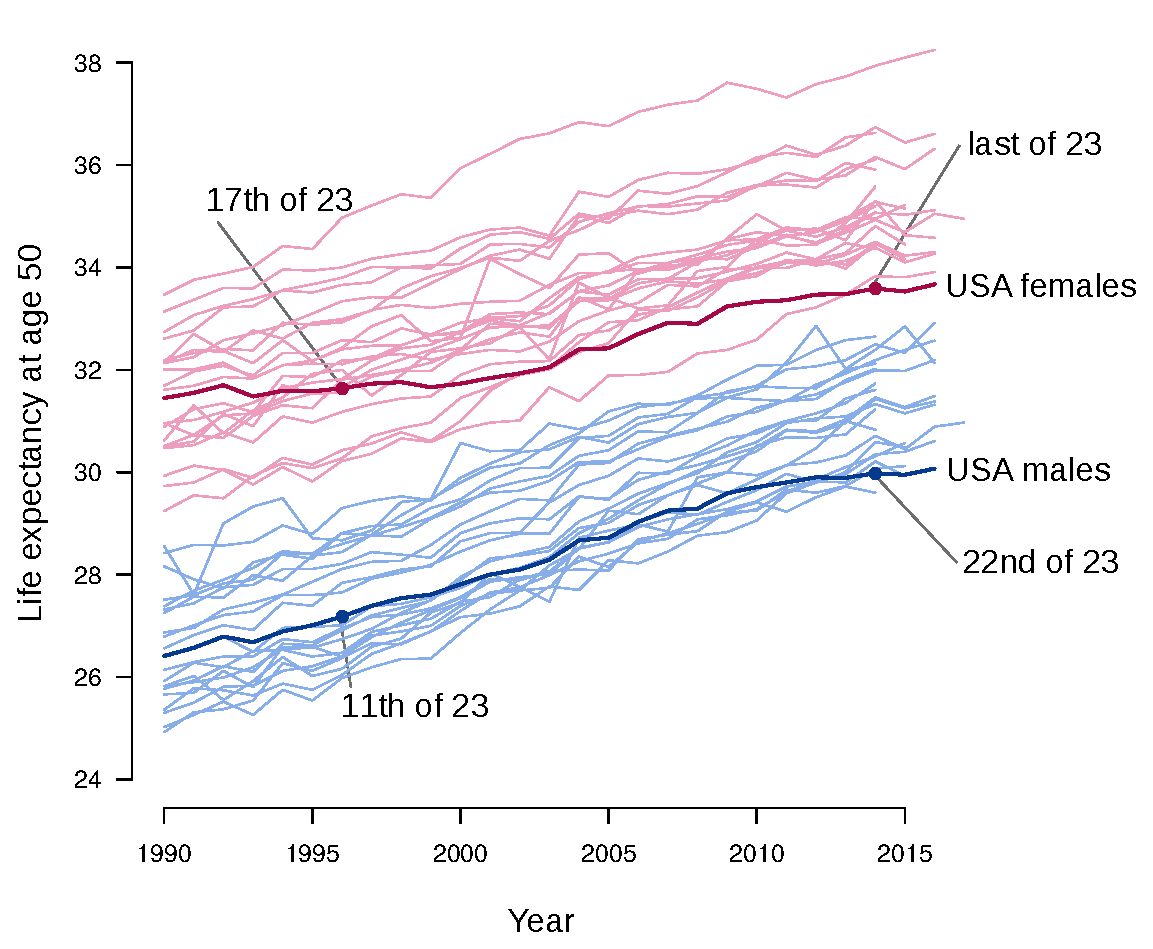
\includegraphics[scale=.7]{Figures/USAvsOthers_Ink.pdf}
\caption{Trends in male and female remaining life expectancy at age 50 from 1990 to 2016 in 23 high-income HMD countries:  \\ \footnotesize Australia, Austria, Belgium, Switzerland, Germany, Denmark, Spain, Finland, France, Ireland, Israel, Italy, Japan, Luxembourg, the Netherlands, Norway, Portugal, Sweden, Taiwan, Great Britain, and the United States. We exclude countries of the former Eastern block, as well as HMD countries without data for the years 1996 and 2014.}
\label{fig:uslose}
\end{figure}

Mean remaining lifespan at age 50 in the USA increased by 2.9 years for males and 2.0 years for females in the two decades from 1996 to 2016, amounting to 10\% and 6\% increases, respectively. In the net, mortality has improved over this period. Despite underperformance in international perspective, there is still some success to account for. Several factors underly this modest improvement, including improved living standards and nutrition over the lifecourse of the cohorts composing the 50+ population, as well as medical improvements allowing for quicker and more certain recovery from many health conditions. Cures, lifesaving, and life-extending treatments may delay the deaths of both healthy and chronically ill or disabled persons, and therefore may contribute to increasing both years lived in a state of morbidity and in good health. For the typical case of population-level death rates that underly estimates of period life expectancy, it is not clear whether a rate improvement comes about due to improvements in the health and wellbeing of a population, the effects of medicine, or the population composition with respect to various kinds of risk sets, such as the educational composition. 

Our objective is to quantify how much of the increase in life expectancy (LE), disabled life expectancy (DLE), and disability-free life expectancy (DFLE) at age 50 is due to 1) changes in the mortality rates of the disabled and disability-free, 2) changes in SES-differential mortality, as captured by education-specific mortality, 3) changes in the fraction in each educational group and the education-specific prevlaence of disability at age 50, and 4) changes in the onset of disability (disablement) and recovery from disability. These effects can be condensed as mortality change, versus disability change, versus compositional change. We consider this question to be of great importance because results will reveal the most important levers in life expectancy change, and these components in turn may indicate the potential for future improvements, but also the culprits of contemporary stagnation. 

Potential improvements may be in store on a 20-year horizon due to compositional differences already determined today in better-educated younger ages, but also due to preventative, technological, and policy changes that affect transitions into and recovery from disability, and that would require investment. Mortality change itself, net of the population breakdown by education and disability status could be due to ongoing improvements in reducing the risk of death. Place your bets now ladies and gentlemen: is it delayed onset, improved recovery, mortality improvement, or compositional change. 

In section~\ref{sec:methods} we briefly describe the data and methods used to answer our main questions. In section~\ref{sec:results} we describe trends in LE, DLE, and DFLE at age 50, and we decompose changes over time in each of these expectancies into effects from changes in disablement, recovery, mortality with and without disability, and changes in the educational composition at age 50. In section~\ref{sec:discussion} we formalize what can be learned from this analysis, how it relates to the literature, and the limitations of our data and research design. We conclude with recommendatinos for further scientific inquiry and for population-level health intervention.

\section{Methods and materials}
\label{sec:methods}
% verbrugge ADL progression could be used as proxy for mild and severe
We estimate disability free and disabled life expectancy using incidence-based discrete-time Markov models. The model separates the population into two groups: disability free and disabled, where disability is defined as having at least one of a set of 5 activities of daily living (ADLs) \footnote{The five ADLs include bathing, eating, dressing, walking across a room, and getting into or out of bed.}. Fig.~\ref{fig:statespace} shows the formal state space used in our model of disability. We use RAND version P of the US Health and Retirement Study \citep{RAND, HRS} to estimate the probabity of transitioning into and out of disability, and the probability of dying with and without disability with multinomial logit models. We stratify models by sex and three educational attainment categories\footnote{Education categories include 1) less than high school, 2) high school, including GED and some college, but no degree, and 3) university degree, including 2-year associates degrees.}, and control for four race and ethnicity categories \footnote{}. Age-effects for two-year age groups from age 50 to 110 (31 age groups) are captured flexibly with splines.\footnote{We use 2-year age groups because HRS waves are spaced two years apart.} With this we obtain point estimates for transition probabilities in the years 1996, 2006, and 2014. 

\begin{figure}[ht!]\centering
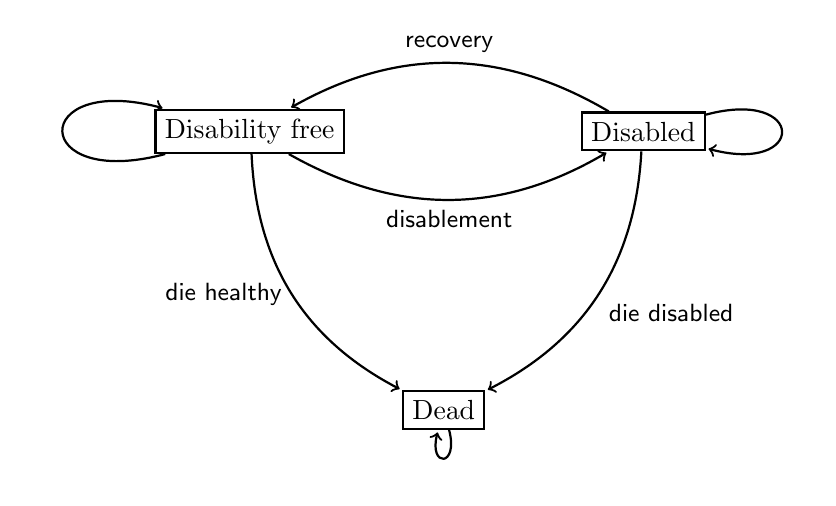
\begin{tikzpicture}[->,shorten >=1pt,auto,node distance=5cm,
  thick,main node/.style={draw}]

  \node[main node] (1) {Disability free};
  \node[main node] (2) [right of=1] {Disabled};
  \node[main node] (3) [below left of=2,xshift=1cm] {Dead};

  \path[every node/.style={font=\sffamily\small}]
    (1) edge [bend right] node [left] {die healthy} (3)
    (1) edge [bend right] node [below] {disablement} (2)
    (1) edge [loop left] node {} (1)
    (2) edge [bend right] node [above] {recovery} (1)
    (2) edge [loop right] node {} (2)
    (2) edge [bend left] node {die disabled} (3)
    (3) edge [loop below] node {} (3);
    
\end{tikzpicture}\\

\caption{State space used for our discrete Markov model. Disabled is defined as having at least one (of a set of five) ADLs. Age transitions are not depicted in the diagram for simplicity. We assume no transitions between education states after age 50, and therefore this is the state space for any given education group.}\label{fig:statespace}
\end{figure}

Given age schedules of transition probabilities depicted in Fig~\ref{fig:statespace} for each educational group and year, as well as the prevalence of disability at age 50 for each educational group and the fraction of the population in each group, the calculation of life expectancy follows a well-known set of matrix calculation steps, which we omit for the sake of brevity. These steps can be captured in a single function, $e^i(\textbf{p},\pi)$, where $e^i()$ defines the average time spent in the $i^{th}$ state (LE, DFLE, or DLE) given a vector of age- and education-specific transition probabilities $\textbf{p}$, and a vector $\pi$ of the fraction of persons aged 50 in each educational group and disability state.\footnote{For a given year and sex, $\textbf{p}$ is of length 744: 31 age groups $\times$ 3 education groups $\times$ 2 states $\times$ 4 transition types. $\pi$ is of length 6: the fraction of the population ata age 50 in 2 states $\times$ 3 education groups.} This functional form facilitates classic demographic decomposition of the change in LE, DFLE, or DLE between two time points (1996 to 2006 and 2006 to 2014) that is due to each element of $\textbf{p}$ and $\pi$. 

We decompose changes over time using the method proposed by \citet{horiuchi2008}, which is general enough and sufficiently stable for our needs and is available in the \texttt{DemoDecomp} \texttt{R} package \citep{DemoDecomp}\footnote{Other options to decompose would be to use the algorithm of stepwise replacement proposed by \citet{andreev2002algorithm}, or by carrying out a lifetable response experiment as proposed by \citet{caswell1989analysis}. The first is equally general and straightforward to set up, but it is sensitive to the order in which elements are replaced, and it does not maintain the identity $p(stay) + p(entry) + p(exit) = 1$ over the algorithm steps. The second is (we conjecture) asymptotically equivalent to the Horiuchi method, but it requires extensive matrix derivations.}. Decomposition produces an estimate of the contribution of each age-specific difference in transition probability and age-50 population fractions (by education and disability state), for a total of $744 + 6 = 750$ elements. These contributions are given in year-units, and we aggregate them in various ways to determine the degree to which changes in each transition type (each edge in the Fig.~\ref{fig:statespace} graph), as well as changes in the prevalence and educational composition of the age-50 population.

[Notes] Confidence intervals on expectancies and decomposition results will come in a later revision of this work. We may consider alternative state space definitions, and change some details with age splines. We may also estimate transition probabilities for each year in order to provide a more detailed time series. 

\section{Results}
\label{sec:results}
\subsection{Transition probabilities and life expectancy}
The transition probilities for females in the year 2006 are given as an example to show the basic characteristics of each age pattern. These are different for each time point, education group, and between the sexes, but the basic schematic shape of each curve is essentially the same for all subgroups: i) mortality increases monontonically for both the disabled and the non-disabled, but is higher for the disabled ii) the probability of staying healthy decreases monotonically after age 50, iii) the probability of staying disabled either remains flat until near the modal age at death, afer which it falls, or else it monotonically falls over all ages, iv) the probability of recovering from disability monotonically falls, and v) the probability of entering into a state of disability first increases strongly, then decreases after age 100 as the force of mortality becomes the dominant transition. 

\begin{figure}[ht!]
\centering
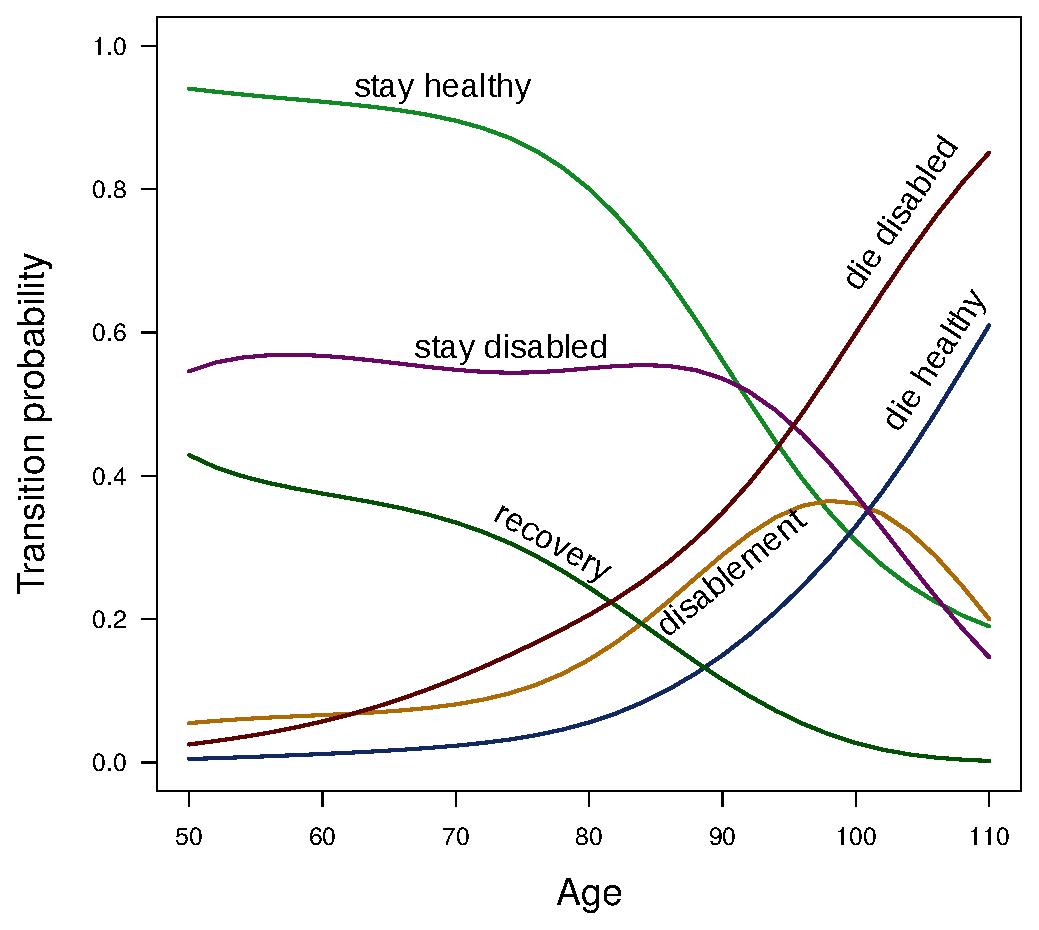
\includegraphics[scale=.7]{Figures/TransitionsInk.pdf}
\caption{Transition probabilities for US females in 2006, as estimated from HRS data, all education groups combined. These age schedules correspond to the arrows in Fig.~\ref{fig:statespace}.}
\end{figure}

The total life expectancies we calculate using HRS data for all education groups combined (and controlling for race and ethnic composition) are very close to the HMD levels and trends, which were based on more aggregate data (See Fig.~\ref{fig:e50}). This gives some assurance that the data and model are working as expected, but one ought not expect the two trends to coincide as a matter of definition: the HRS estimates refer to a statistical centroid of race/ethnicity and education groups, with prevalence having arrived at its steady state given the HRS transition probabilities: the real world underlying HMD estimates is a messy composition and it is not in a steady state, and so we expect some departures, even under perfect data conditions. Also of interest to our study is the size of the educational gradient: we observe an approximately 6-year gap between the highest and lowest educated, which has been increasing for both males and females. This gap size is roughly consistent with \citet{montez2014cumulative}, whose model differs from our own in several ways.

\begin{figure}[ht!]
\centering
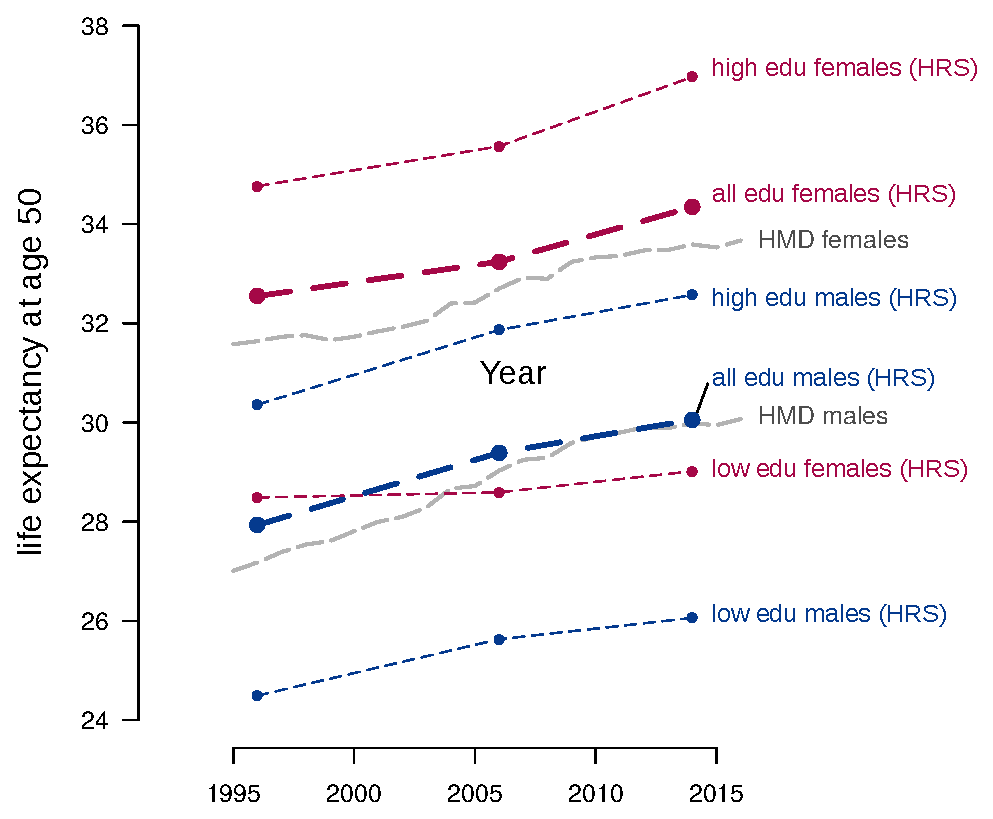
\includegraphics[scale=.7]{Figures/e50_Ink.pdf}
\caption{Life expectancy at age 50 for males (blue) and females (purple) using HRS transition probabilties. Bold dashed lines indicate the HRS estimate for all educational groups combined. It is quite close to the HMD estimate (gray background lines). High education (low education) groups in light dashed lines have approximately three years higher (lower) values than the average for both males and females.}
\label{fig:e50}
\end{figure}

\subsection{Life expectancy with and without disability}

Life expectancy breaks down into two additive expectancies, DFLE and DLE, which we show in Fig.~\ref{fig:barsmales} for males and in Fig.~\ref{fig:barsfemales} for females. We show the breakdown for all education groups combined (Fig.~\ref{fig:barsmalesa} and ~\ref{fig:barsfemalesa}), where the total length of each bar corresponds to the bold dashed point estimates in Fig.~\ref{fig:e50}. For both males DFLE increased from 1996 to 2006 to 2014. For females DFLE increased by more than a year in the first period, but stagnated in the second period, even falling by \rd{0.2} years in the low educated group. DLE also increased for each education group over time, and the fraction of life expectancy at age 50 in the state of disability increased by less than a percentage point over the whole period for males, and by an average of about \rd{1 percentage point} for females. Sex differences are also as expected from the literature: DFLE is \rd{5-12\%}, and DLE is \rd{35-70\%} higher for females than for males within each year and education group. Notably, most of the increase in LE for females from 2006 to 2014 was due to a \rd{1.27} year increase in DLE (all education combined). 

\begin{figure}[ht!]
    \centering
    \begin{subfigure}[b]{0.2\textwidth}
        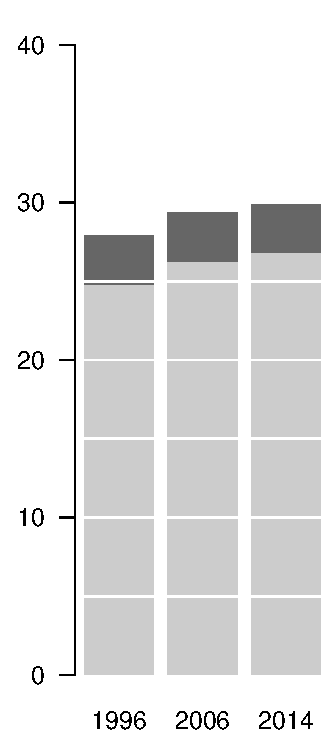
\includegraphics[scale=.5]{Figures/bar_male_all.pdf}
        \caption{All education}
        \label{fig:barsmalesa}
    \end{subfigure}
    ~ %add desired spacing between images, e. g. ~, \quad, \qquad, \hfill etc. 
      %(or a blank line to force the subfigure onto a new line)
    \begin{subfigure}[b]{0.2\textwidth}
        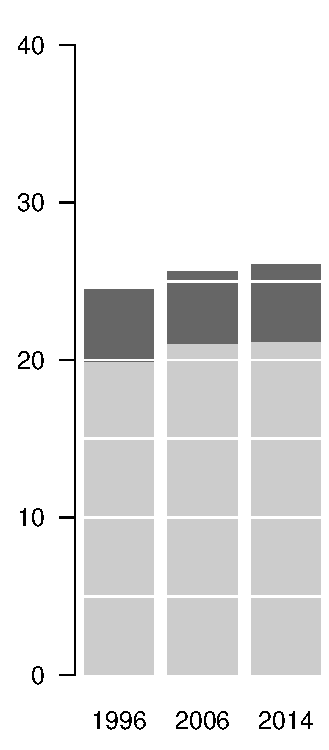
\includegraphics[scale=.5]{Figures/bar_male_pri.pdf}
        \caption{Low education}
    \end{subfigure}
    ~ %add desired spacing between images, e. g. ~, \quad, \qquad, \hfill etc. 
    %(or a blank line to force the subfigure onto a new line)
    \begin{subfigure}[b]{0.2\textwidth}
        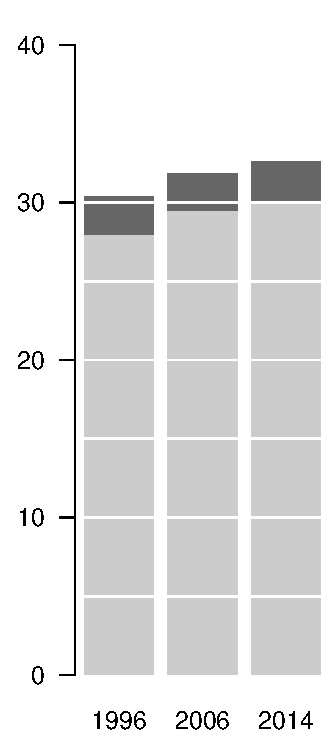
\includegraphics[scale=.5]{Figures/bar_male_uni.pdf}
        \caption{High education}
    \end{subfigure}
    \caption{Male DFLE (light gray) and DLE (dark gray) for all education combined (a), for the low-educated (b) and the high-educated (c) subgroups in 1996, 2006 and 2014. Both DFLE and DLE have increased steadily for each education grouping.}\label{fig:barsmales}
\end{figure}

\begin{figure}[ht!]
    \centering
    \begin{subfigure}[b]{0.2\textwidth}
        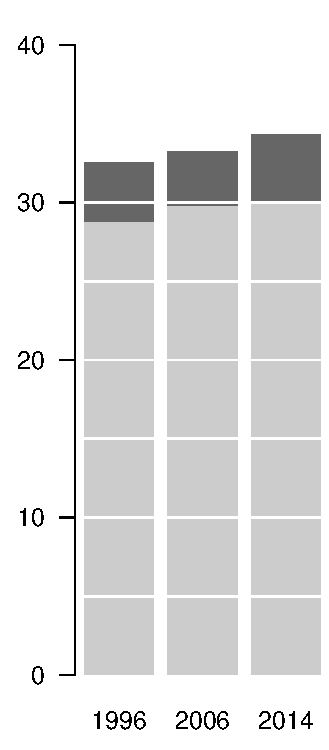
\includegraphics[scale=.5]{Figures/bar_fem_all.pdf}
        \caption{All education}
        \label{fig:barsfemalesa}
    \end{subfigure}
    ~ %add desired spacing between images, e. g. ~, \quad, \qquad, \hfill etc. 
      %(or a blank line to force the subfigure onto a new line)
    \begin{subfigure}[b]{0.2\textwidth}
        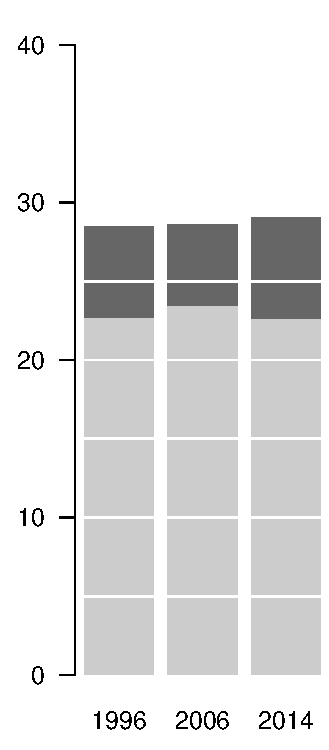
\includegraphics[scale=.5]{Figures/bar_fem_pri.pdf}
        \caption{Low education}
    \end{subfigure}
    ~ %add desired spacing between images, e. g. ~, \quad, \qquad, \hfill etc. 
    %(or a blank line to force the subfigure onto a new line)
    \begin{subfigure}[b]{0.2\textwidth}
        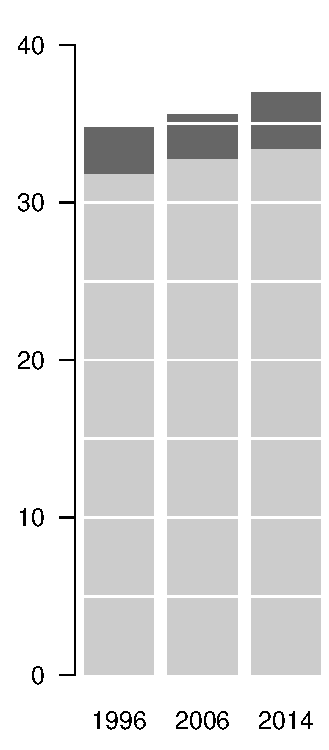
\includegraphics[scale=.5]{Figures/bar_fem_uni.pdf}
        \caption{High education}
        \label{fig:barsfemalesc}
    \end{subfigure}
    \caption{Female DFLE (light gray) and DLE (dark gray) for all education combined (a), for the low-educated (b) and the high-educated (c) subgroups in 1996, 2006 and 2014. Both DFLE and DLE have increased for each education grouping, but the increase in DFLE was trivial for the most recent period.}\label{fig:barsfemales}
\end{figure}

\subsection{Decomposition results}
The change in the value of LE, DFLE, and DLE from 1996 to 2006 and from 2006 to 2014 is decomposed and summarized in Tab.~\ref{tab:males} and Tab.~\ref{tab:females}, with table shading to indicate the magnitude and direction of effects (green for improvement, purple for deterioration, darker for higher magnitudes). Each cell value has been summed over age. Each table is interpreted as follows: the lower right corner gives the total change in LE for the period, which is the sum of the change in DLE and DFLE (Total margin). The contribution of each transition to each expectancy change is given in the rows labeled onset (disablement), die healthy (disability free), recovery, and die disabled.

From Tab. 1a we see that most of the \rd{1.41} year increase in LE was due to improved among those with no disability, adding \rd{11} months to DFLE and \rd{2.5} months to DLE, respectively. In general, mortality improvements in any state contribute to increases in the expectancy of all states. Onset among males improved in both periods, and this adds nearly twice as many years to DFLE as it deducts from DLE. Recovery from disability worsened trivially in the first period, and importantly in the second period, adding \rd{two months} to DLE and deducting \rd{four months} from DFLE. We might call the net effect of onset and recovery something like `health dynamics', in which case health dynamics added \rd{1.5} months to LE in the first period and deducted \rd{a} month from LE in the second period. Most change was positive and due to mortality. Had recovery remained unchanged in the second period, we might have seen a \rd{XXX} increase in LE.

\rd{[enter description of structural effect here]}


\begin{table}[!ht]
      \caption{Males (all education combined). Contributions of changes in each transition to the change in each expectancy.}
      \label{tab:males}
      \centering
\subfloat[][1996-2006]{
      \begin{tabular}{rrr|r}
      \input{Data/Tables/mspec06/m-1996-2006-all.tex}
     \end{tabular}
}
     \qquad
\subfloat[][2006-2014]{
      \begin{tabular}{rrr|r}
      \input{Data/Tables/mspec06/m-2006-2014-all.tex}
     \end{tabular}
}
\end{table}
\rd{[education composition component forthcoming]}


\begin{table}[!ht]
      \caption{Females (all education combined) Contributions of changes in each transition to the change in each expectancy.}
      \label{tab:females}
      \centering
\subfloat[][1996-2006]{
      \begin{tabular}{rrr|r}
      \input{Data/Tables/mspec06/f-1996-2006-all.tex}
     \end{tabular}
}
     \qquad
\subfloat[][2006-2014]{
      \begin{tabular}{rrr|r}
      \input{Data/Tables/mspec06/f-2006-2014-all.tex}
     \end{tabular}
}
\end{table}

Trends for females have also been dominated by mortality improvements of the non-disabled, adding \rd{ten} months to LE in the first period and \rd{1.36} years in the second period, most of which acrued to DFLE. Mortality of the disabled population deteriorated in the first period and recovered in the second period, for a net increase of \rd{one month} in LE. Onset improved in the first period, deducting \rd{five} months from DLE and adding \rd{nine} months to DFLE. In the second period onset stagnated, and more importantly recovery deteriorated so much as to add \rd{half a year} to DLE and deduct \rd{11 months} from DFLE. In the net, health dynamics worsened slightly from 1996 to 2014, deducting \rd{a month} from LE. Most of the improvement in female life expectancy at age 50 was due to increased DLE, making this a period of disability expansion, driven entirely by a setback in recovery from disability.


\section{Discussion}
\label{sec:discussion}
Our decomposition results show that over the 19 years from 1996 to 2014 net health dynamics worked to keep disabled life expectancy in dynamic equilibrium, consistent with \citet{manton1982changing} and others. Disability expansion ocurred for females over the whole period studied not due to changes in health dynamics, which acted to deduct \rd{half a year} from DLE from 1996 to 2006, and then add \rd{half a year} to DLE from 2006 to 2014. Mortality deterioration of the disabled population in the first period was offset by mortality improvements in the second period, leaving the final net increase in DLE from 1996 to 2014 almost entirely due to mortality improvements of the non-disabled population. Mortality improvements are unequivocally good, whether they lead to disability expansion or compression. The best levers for interventions with respect to the time and fraction of life spent disabled are those that influence onset and recovery of disability.

We show that \rd{X\%} of the increase in life expectancy at age 50 was due to an increase in the educational attainment of 50-year-olds. This lever is very strong because the educational gradient for each of the transition types in our model is steep and has become steeper over time.

\rd{Mikko: A key point in the discussion can be that that this paper considers the DFLE/DLE dynamics from a novel perspective, although the perspective is perhaps obvious for demographers:  decomposition of the change to contributions to onset, recovery, and death. Has someone done this? If not let’s be very bold about that. If someone has done this, surely they have not done this using recent high-quality U.S. data. So either we are the first to do this, or we are the first to do this in our current context in which understanding DFLE/DLE dynamics is particularly important.}

\rd{Some useful references
\url{https://link.springer.com/content/pdf/10.1353\%2Fdem.0.0070.pdf} – a key paper, as is also the Montez/Hayward 2014 paper. Incidence based markov models, ADL disability, 1984-2000. The paper has conclusions that sound as if they did what we do: “Changes in disability-free life expectancy resulted from decreases in disability incidence and increases in the incidence of recovery from disability across the two survey cohorts. Age-speci c mortality among the ADL disabled declined signicantly in the later cohort after age 80. Mortality for the IADL disabled and the nondisabled did not change signicantly” However, they don’t decompose. These conclusions are based on eyeballing of incidence/recovery/death trajectories at two time points. This perhaps gives some leverage to our motivation: Crimmins et al. did a “decomposition” with incidence based models but arrived at a conclusion that is opposite to ours, perhaps because of the difference in the “decomposition” methods.
 
Plenty of Sullivan papers that are related, here just a few
 
\url{https://ajph.aphapublications.org/doi/abs/10.2105/AJPH.2016.303089} -- Sullivan, 1982-2004, finds that in particular for women improvements in LE are largely DLE (no DFLE), and calls for policies that would *postpone* disability. This is perhaps in contrast to what we find, that improvements in DFLE stem largely from keeping the DF alive, and that investing in recovery may deliver largest gains in DFLE
 
\url{https://link.springer.com/article/10.1007/s11113-014-9337-6}-- Sullivan, NHIS data, 1991-2001, interesting finding that “The 1990s was a period where the increased years of life between ages 60 and 90 were concentrated in disabled years for most population groups.”
 
\url{http://www.nber.org/papers/w22306}  -- Chernew, Cutler et al use data over 1992-2008, ADL for disability and Sullivan type approach although they talk about incidence (they don’t cite Sullivan, and write as if they invented the method), and find that CVD and vision problems explain about 2/3 of the improvement in DFLE. I am not sure how any of this translates into our analysis, since their focus is on specific conditions that results in people having ADL. But can say decompositions in the Sullivan framework have been attempted.}
%There are obvious ways to frame these results in a compression, expansion, equilibrium language. That may be nice because it's familiar language. To be clear it would be possible to decompose with respect to a clear measure of compression (DLE / LE), but I do prefer to keep things in year units.

%It would also be possible to plug in some counterfactuals to guage better what levers are the closest at hand. In the way things are now, it would seem to pay off nicely to invest in recovery: improvements in recovery adds more to DFLE than it subtracts from DLE. This is probably truer the greater the mortality gradient between states. I've also asked DCS to add a state ``healthy but ever disabled'', as a check on the homogeneity of the healthy-- this is necessary to know how realistic the recovery payoff, as stated above, is. It would change the arrow configuration in the state space too (no returns to straight good health).

\section{Conclusions}
\label{sec:conclusions}
% bibliography
\bibliographystyle{spbasic}
\bibliography{references}  
\end{document}



%This is a tabular representation of the decompositon results that were represented as bar charts in the REVES talk. I think it took too much mental gymnastics at REVES to realize the various ways in which things are additive, but it is actually quite clear in the following tables, since we have marginal sums, and people are used to such tables. First, we have a pretty good match to the HMD LE trend for the US (not shown).\footnote{Potential departures could be due to several understandable factors, and can be explained if necessary, but it's not worth gettign sidetracked by that just now.}. 

%The main goods are the decompositions of the within-group changes between our present 3 time points (1996, 2006, 2014). Those time points are willy nilly, and we may move to annual estimates soon, so we can select years at-will. First, note that the columns DFLE and DLE sum to LE, both within changes due to transiton rates and within state expectancy changes. To interpret signs, it helps to moralize some: We \emph{want}: mortality down (DFLE +, DLE +), transitions to disability down (DFLE+, DLE-), and recovery up (DFLE+, DLE-).

%The total change in male LE from \textbf{1996 to 2006} was 1.41, of which 1.27 came from an overall increase of 1.27 in DFLE. Looking at the LE column, we see that transitions from healthy to dead (m14) account for most of the change. Looking at the DLE column, we see that most increases were also due to the decreased mortality of healthy people (m14), but this was offset almost entirely by decreaed entries to disability (m12), not bad! The mortality of the disabled also improved a bit, adding .09 to DLE, .07 to DFLE (by allowing people to cycle back by not dying), adding to .15 LE, also a good outcome.

%The total change in male LE from \textbf{2006 to 2014} was .65, of which .38 came from an increase in DFLE, and .27 from DLE, a less optimal breakdown. Looking at the LE column, we see that transitions from healthy to dead (m14) account for most of the change. The other story in this table is reduced recovery, which of course steals more healthy years than it adds disabled years. The other two factors increasing DLE are things that are actually quite good: they survive better, as do healthy people, allowing them to become disabled. Transitions into disability actually decreased. So, although DLE increased, most of the story behind it is straight good news: we just know that recovery is the only setback. Make sense?

%For females from \textbf{1996 to 2006} there was a modest gain in LE of .76 years, due to a strong increase in DFLE, partially offset by a decrease in DLE. Sounds like a good tradeoff until we realize that the reduction in DLE was due to i) worse mortality and ii) worse recovery. At the same time transitions to disability decreased, adding .73 to DFLE and deducting .43 from DLE- that's straight good news, but transitinos out of disability were straight bad news. This is not the way to engineer compression folks. The main protagonist here is again improved mortality of the healthy.

%For females from \textbf{2006 to 2014} we have a strong increase in LE of 1.47 years, due entirely to mortality (1.36+.54), mostly the mortality of the healthy. Recovery got way worse (-.93,+.51)and onset was unchanged. This lead to a large increase in DLE and a merely modest increase in DFLE: so large was the recovery setback (-.93) that it almost entirely chancelled out the good news for the mortality of the healthy (+.98). If we could ignore ``health dynamics'', we would have had something like dynamic equilibrium in this period, but althogether this is straight expansion, boo.